\section{Chọn ổ lăn trục 1}
\subsection{Chọn trước ổ}
\begin{figure}[H]
    \centering
    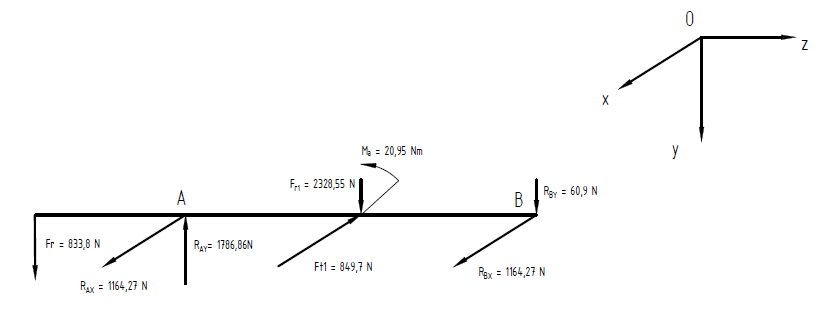
\includegraphics[width=1\textwidth]{pictures/tinholan1.png}
\end{figure}
Xác định phản lực tại các vị trí A và B:
\[
    F_{rA} = \sqrt{R_{AX}^2 + R_{AY}^2} = \sqrt{1164,27^2 + 1786,86^2} = 2132,7N
\]
\[
    F_{rB} = \sqrt{R_{BX}^2 + R_{BY}^2} = \sqrt{1164,27^2 + 60,9^2} = 1165,86N
\]
Tại vị trí A có lực tập trung lớn hơn nên ta chọn ổ lăn theo vị trí A của trục I.
\[
    \frac{F_a}{F_r} = \frac{765,588}{2132,7} = 0,359
\]
Vì $0,3 < \frac{F_a}{F_r} = 0,36 < 0,7$ nên ta chọn loại ổ bi đỡ là ổ bi đỡ chặn 1 dãy. \\
Ta có đường kính trục tại ổ lăn: d = 25mm \\
$\Rightarrow$ Chọn ổ lăn loại ổ bi đỡ chặn, cỡ trung có ký hiệu 46305 với $C = 21100N$ và $C_o = 14900N$.
\begin{figure}[H]
    \centering
    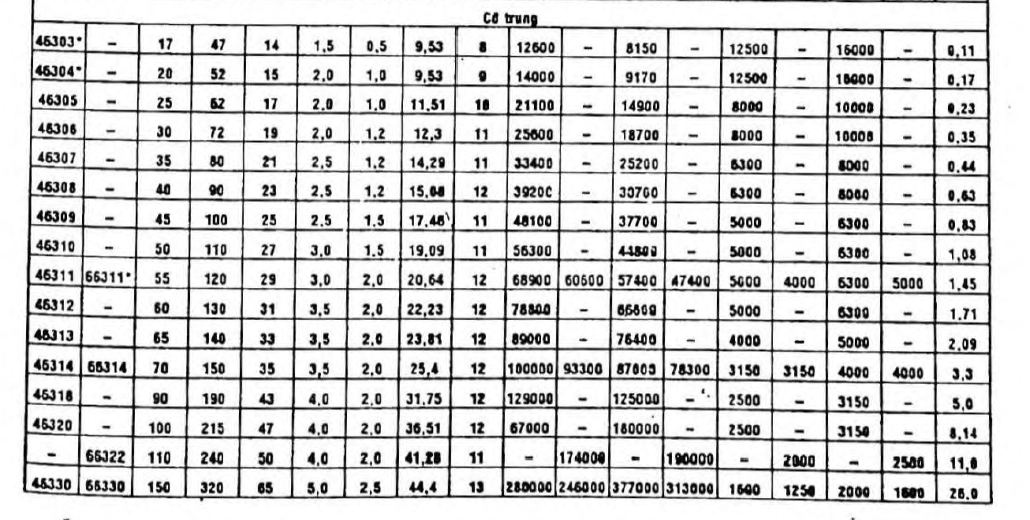
\includegraphics[width=1\textwidth]{pictures/chono1.png}
    \caption{Tiêu chuẩn chọn ổ đỡ chặn cỡ trung}
\end{figure}
\subsection{Tính ổ lăn theo khả năng tải trọng}
\subsubsection*{Chọn các hệ số}
\begin{itemize}
    \item Chọn hệ số $K_\alpha = 1$ do tải trọng tĩnh.
    \item Chọn hệ số $K_t = 1$ do làm việc ở nhiệt độ thường.
    \item Chọn hệ số $V = 1$ do vòng trong quay.\\
    Chọn hệ số X và Y: \\
    $\frac{F_a}{C_o} = \frac{765,588}{14900} = 0,0514 \Rightarrow$ chọn e = 0,34.\\
    $\frac{F_a}{VF_r} = \frac{765,588}{1.2132,7} = 0,359 > e = 0,34$ nên chọn X = 0,45 và Y = 1,62.
\end{itemize}
\subsubsection*{Thời gian làm việc tính bằng triệu vòng quay}
\[
    L = \frac{60L_hn}{10^6} = \frac{60.6.280.8.2.482,5}{10^6} = 778,176 
\]
\cleardoublepage
\subsubsection*{Tải trọng quy ước tác dụng lên ổ lăn}
\[
    Q = (XVF_r+YF_\alpha)K_\sigma K_\tau = (0,45.1.2132,7 + 1,62.765,588).1.1 = 2200N
\]
\[
    C_t = Q\sqrt[m]{L} =2200\sqrt[3]{778,176} = 2200.11,5 = 20235,6N
\]
Vì $C_t < C = 21100N$ nên việc chọn cỡ nhẹ là hợp lý.
\begin{center}
\begin{tabular}{|c|c|c|c|c|c|c|c|}
    \hline
       \textbf{Ký hiệu} & \textbf{d, mm} & \textbf{D, mm} & \textbf{B, Nm} & \textbf{r, mm} & \textbf{C, N} & \textbf{$C_o$, N} & \textbf{$L_h$, giờ} \\
    \hline
    46305 & 25 & 52 & 17 & 2 & 21100 & 14900 & 26880 \\
    \hline
\end{tabular}
\end{center}
\section{Chọn ổ lăn trục 2}
\subsection{Chọn trước ổ}
\begin{figure}[H]
    \centering
    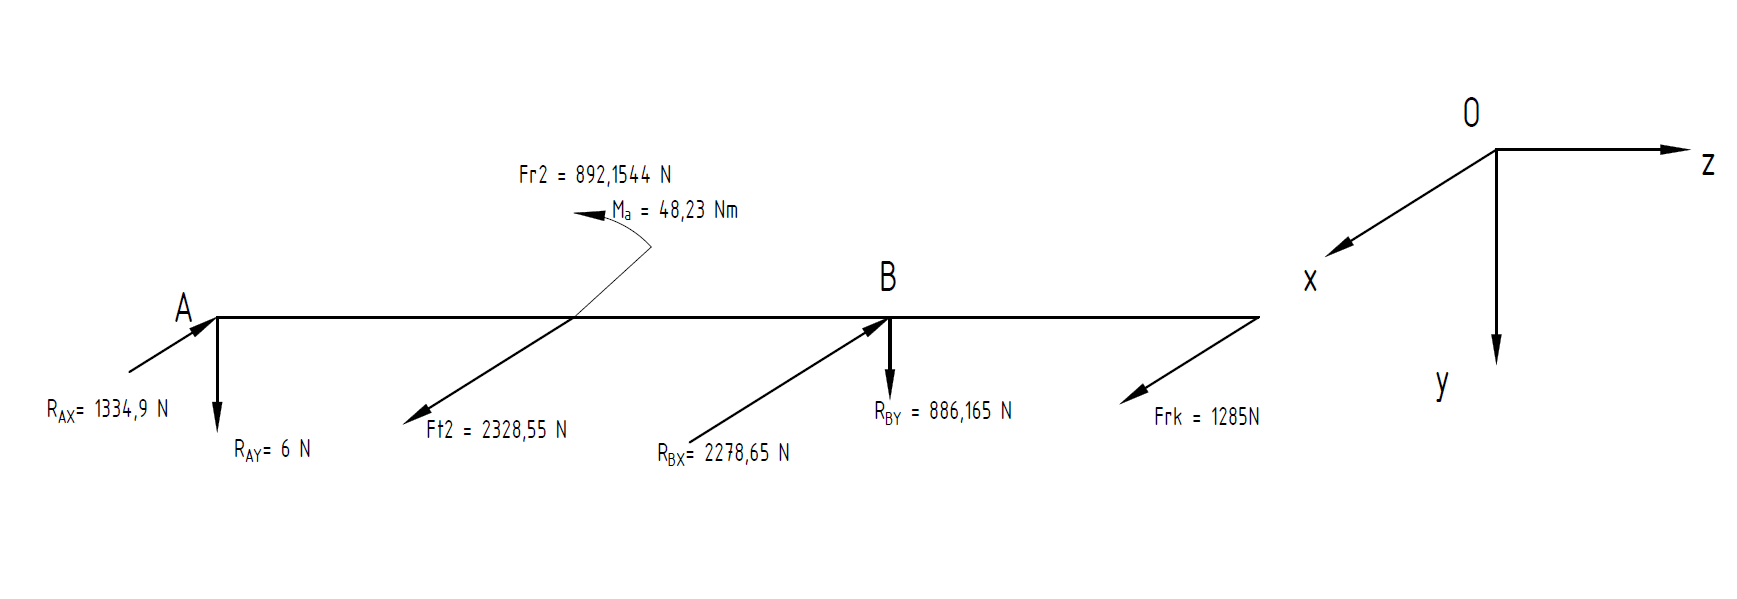
\includegraphics[width=1\textwidth]{pictures/tinholan2.png}
\end{figure}
Xác định phản lực tại các vị trí A và B:
\[
    F_{rA} = \sqrt{R_{AX}^2 + R_{AY}^2} = \sqrt{1334,9^2 + 6^2} = 1334,9N
\]
\[
    F_{rB} = \sqrt{R_{BX}^2 + R_{BY}^2} = \sqrt{2278,65^2 + 886,165^2} = 2444,9N
\]
Tại vị trí B có lực tập trung lớn hơn nên ta chọn ổ lăn theo vị trí B của trục II.
\[
    \frac{F_a}{F_r} = \frac{765,588}{2444,9} = 0,313
\]
Vì $0,3 < \frac{F_a}{F_r} = 0,36 < 0,7$ nên ta chọn loại ổ bi đỡ là ổ bi đỡ chặn 1 dãy. \\
Ta có đường kính trục tại ổ lăn: d = 45mm \\
$\Rightarrow$ Chọn ổ lăn loại ổ bi đỡ chặn, cỡ siêu nhẹ có ký hiệu 46109 với $C = 17300N$ và $C_o = 13700N$.
\begin{figure}[H]
    \centering
    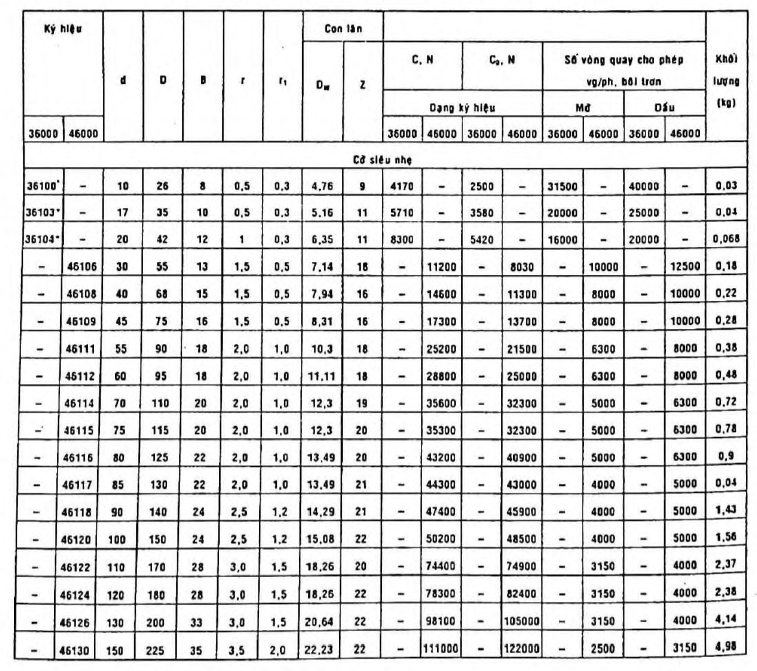
\includegraphics[width=1\textwidth]{pictures/chono2.png}
    \caption{Tiêu chuẩn chọn ổ đỡ chặn cỡ siêu nhẹ}
\end{figure}
\subsection{Tính ổ lăn theo khả năng tải trọng}
\subsubsection*{Chọn các hệ số}
\begin{itemize}
    \item Chọn hệ số $K_\alpha = 1$ do tải trọng tĩnh.
    \item Chọn hệ số $K_t = 1$ do làm việc ở nhiệt độ thường.
    \item Chọn hệ số $V = 1$ do vòng trong quay.\\
    Chọn hệ số X và Y: \\
    $\frac{F_a}{C_o} = \frac{765,588}{13700} = 0,056 \Rightarrow$ chọn e = 0,37.\\
    $\frac{F_a}{VF_r} = \frac{765,588}{1.2444,9} = 0,313 < e = 0,37$ nên chọn X = 1 và Y = 0.
\end{itemize}
\subsubsection*{Thời gian làm việc tính bằng triệu vòng quay}
\[
    L = \frac{60L_hn}{10^6} = \frac{60.6.280.8.2.76,6}{10^6} = 123,54 
\]
\subsubsection*{Tải trọng quy ước tác dụng lên ổ lăn}
\[
    Q = (XVF_r+YF_\alpha)K_\sigma K_\tau = (1.1.3213,53 + 0.765,588).1.1 = 3213,53N
\]
\[
    C_t = Q\sqrt[m]{L} =3213,53\sqrt[3]{123,54} = 3213,53.11,5 = 160005N
\]
Vì $C_t < C = 17300N$ nên việc chọn cỡ siêu nhẹ là hợp lý.
\begin{center}
\begin{tabular}{|c|c|c|c|c|c|c|c|}
    \hline
       \textbf{Ký hiệu} & \textbf{d, mm} & \textbf{D, mm} & \textbf{B, Nm} & \textbf{r, mm} & \textbf{C, N} & \textbf{$C_o$, N} & \textbf{$L_h$, giờ} \\
    \hline
    46109 & 45 & 75 & 16 & 1,5 & 17300 & 13700 & 26880 \\
    \hline
\end{tabular}
\end{center}
\cleardoublepage